\documentclass{article}
\usepackage[utf8]{inputenc}
\usepackage[T1]{fontenc}
\usepackage{geometry}
\usepackage{graphicx}

\geometry{margin=0.5in}

\begin{document}
\section*{Task}
\subsection*{\underline{Application of Two DAC Converters – XY Control}}
In the microprocessor-based laboratory system, there are three DAC (Digital-to-Analog Converter) units: two inside the processor (DAC\_0 and DAC\_1) and one external DAC (AD7524) connected to port P2. The task is to write a procedure that allows drawing (moving a spot) on an oscilloscope screen of a geometric figure specified by the instructor, such as a \textbf{rhombus, triangle, initials} etc.
\begin{center}
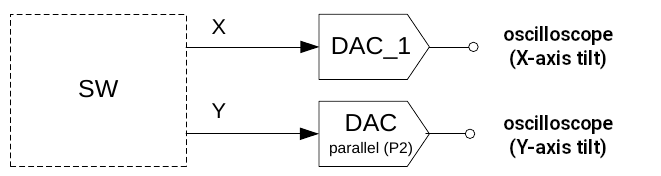
\includegraphics[width=0.7\textwidth]{"../img/DACs_XY_1.png"}
\end{center}
Since the specified figures consist of straight line segments (first-order linear equations), the \underline{recommended} method for drawing is to calculate the Y value based on the equation of the respective segment f(X) within appropriate intervals of the X variable. \\
Other methods can also be used, such as using tables containing the coordinates of points describing the chosen figure on the XY plane.
\vspace{5mm}

The full range of X and Y values is as follows: \\
X -> 00h–FFh or 000h–FFFh depending on the chosen resolution of DAC\_1. \\
Y -> 00h–FFh, based on the 8-bit resolution of the AD7524 DAC. \\
It is also possible to swap the DACs controlling the X and Y axes.
\vspace{5mm}

The first step of the laboratory task will be to draw a straight line as shown in the diagram below.
\begin{center}
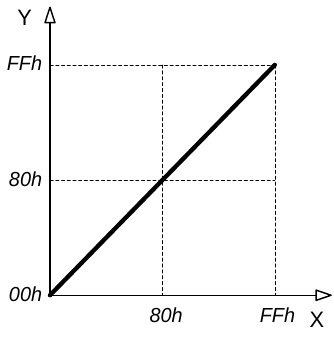
\includegraphics[width=0.5\textwidth]{"../img/DACs_XY_2.png"}
\end{center}

\newpage
\subsection*{\underline{Notes}}
\begin{enumerate}
    \item The image on the oscilloscope screen will be visible if the spot moves along the drawn trajectory cyclically, at the highest possible frequency. Therefore, you need to set the maximum frequency for the DCO system clock or switch the MCLK and SMCLK clock signals to the activated XT2 quartz oscillator, according to the procedure provided below.
\begin{verbatim}
;---------- Basic Clock Module Initialisation --------------------------------------
; - switch from DCO to XT2
; - MCLK & SMCLK supplied from XT2, ACLK = n/a
; - the DCO is left runing
        bis.b   #OSCOFF, SR             ; turn OFF osc.1
        bic.b   #XT2OFF, BCSCTL1        ; turn ON osc.2
BCM0    bic.b   #OFIFG, &IFG1           ; clear OFIFG
        mov     #0FFFFh, R15            ; delay (waiting for oscilator start)
BCM1    dec     R15                     ; delay
        jnz BCM1                        ; delay
        bit.b   #OFIFG, &IFG1           ; test OFIFG
        jnz     BCM0                    ; repeat test if needed
                                        ; MCLK
        bic.b   #040h, &BCSCTL2         ; select XT2CLK as source
        bis.b   #080h, &BCSCTL2         ;
        bic.b   #030h, &BCSCTL2         ; MCLK=source/1 (8MHz)
                                        ; SMCLK
        bis.b   #SELS, &BCSCTL2         ; select XT2CLK as source
        bic.b   #006h, &BCSCTL2         ; SMCLK=source/1 (8MHz)
;---------------------------------------------------------------------------------
\end{verbatim}
    \item Below is an example of \textbf{DAC\_0} configuration (also presented during the lecture). The same configuration should be applied to DAC\_1, which is used in the task.
\begin{verbatim}
;.................................................................. ;DAC_0 initialisation
    bis.w #REFON+REF2_5V, &ADC12CTL0; Reference generator ON, VRef+=2.5V
    bic #DAC12SREF0, &DAC12_0CTL    ; set Vref=VREF+
    bic #DAC12SREF1, &DAC12_0CTL    ;
    bic #DAC12RES, &DAC12_0CTL      ; 12-bit resolution
    bic #DAC12LSEL0, &DAC12_0CTL    ; Load mode 0
    bic #DAC12LSEL1, &DAC12_0CTL    ;
    bis #DAC12IR, &DAC12_0CTL       ; Full-Scale=1xVref
    bis #DAC12AMP0, &DAC12_0CTL     ; High speed amplifier output 
    bis #DAC12AMP1, &DAC12_0CTL     ;
    bis #DAC12AMP2, &DAC12_0CTL     ;
    bic #DAC12DF, &DAC12_0CTL       ; Data format - straight binary 
    bic #DAC12IE, &DAC12_0CTL       ; Interrupt disabled 
    bis #DAC12ENC, &DAC12_0CTL      ; DAC_0 conversion enabled 
;---------------------------------------------------------------------------------
\end{verbatim}
\end{enumerate}

\textit{I assume that I do not need to explain XY control applications further.}
\end{document}